\section{Linkages}
\begin{figure}[!htbp]
 \begin{center}
  \includegraphics{graphics/HumanTurkeyLinkage.pdf}
  \caption{Here are skeleton drawings of a human and a turkey.  When animating skeletons, one tends to make sure that the lengths of the skeleton segments are kept the same length throught the animation.  Otherwise, the animation may depart from what is ideally understood of skeletal motions.}
 \end{center} 
\end{figure}

When graph drawings model physical objects, other qualities avout the graph can be contextualized in a geometric sense.  
Distance, angular relationstips and other geometric qualities of the drawings can be other useful properties of the drawing to perform analysis on.
The \textit{length assignment} of a graph $G=(V,E)$ is $\ell:E \mapsto \bbr^+$. 
For simple graphs, length assignment must be strictly positive, otherwise it may result in two distinct vertices with the same coordinates.
A \textit{linkage} is a graph $G = (V,E)$ with a length assignment $\ell:E \mapsto \bbr^+$.  
Length assignments can be thought of as a metric where $\ell(u,v) = \ell(v,u)>0$.
%Inser linkage here

Consider embeddings of a graph that respects the length assignment.  
A \textit{realization} of a linkage, $(G,\ell)$, is an embedding of a graph, $\Pi$, such that for every edge $\{u,v\} \in E$, $\ell\left( \{u,v\} \right) = \left\vert \Pi(u) - \Pi(v) \right\vert = \left\vert \Pi(v) - \Pi(u) \right\vert$.  
A \textit{plane realization} is a plane embedding with the property, $\ell\left( \{u,v\} \right) = \left\vert \Pi(u) - \Pi(v) \right\vert$.
First let's define the space of realizations for a corresponding linkage, i.e.:
$$P_{(G,\ell)} = \set{\Pi_{(G,\ell)}}{\forall \{u,v\} \in E\text{, }\ell\left( \{u,v\} \right) = \left\vert \Pi(u) - \Pi(v) \right\vert}$$
With respect to $P$, we can establish a \textit{configuration space} that allows one to study problems of motion.  For each vertex of $G$, the embedding of the vertex lies in the plane, i.e. $\Pi(v) \in \bbR^2$.  By enumerating each vertex of $G$, e.g. $v_1, v_2, \dots, v_k, \dots, v_{n}$, we can create a projection mapping from $\mu: P \mapsto \bbR^{2\vert V \vert}$ where the corresponding coordinates of $\Pi(v_k)$ are in the $(2k)^\text{th}$ and $(2k+1)^{th}$ coordinates in $\bbR^{2\vert V \vert}$.  The configuration space is $\mu(P)$.  

Using standard definitions from real analysis, we can begin to pose problems about linkages with respect to a corresponding configuration space.  
We define a path $\gamma: [0,1]\mapsto \mu(P)$ where $\gamma(0)$ corresponds the the projection of a realization of a linkage $\Pi_0$ and $\gamma(1)$ corresponds to another realization of a linkage $\Pi_1$.  
If for any two elements $a,b \in \mu(P)$ that there exists a continuous path $\gamma$ such that $\gamma(0)=a$ and $\gamma(1)=b$, $\mu(P)$ is said to be path connected.   
For $\gamma$ to be continuous we would have that for every $\epsilon > 0$, there exists a $\delta >0$ such that if $x,y \in [0,1]$ and $\vert x-y \vert <\delta$ then $\vlr{\vlr{\gamma(x)-\gamma(y)}}<\epsilon$.
$\gamma$ can be thought of as an animation of drawings that starts at $\gamma(0)$ and ends at $\gamma(1)$
To ask if $\mu(P)$ is a connected space, is to ask if $\mu(P)$ is connected in $\bbR^{2\vert V \vert}$.
By Carpenter's Rule theorem, every realization of a linkage can be continuously moved (without self-intersection) to any other realization \cite{CDR03,Str05}.
In other words, the realization space of such a linkage is always connected.

% \subsection{Configuration Spaces of Linkages}

% \textbf{NOTE THAT THIS SUBSECTION MAY HAVE REPEATED CONTENT}

% Let's focus on the space of embeddings of a linkage. If there are $n$ vertices of a linkage, 
% the \textit{configuration space} of a linkage is said to be a vector space of dimension $2 \cdot n$ 
% where edge length is preserved.  

% A \textit{configuration space} for a linkage $G$ and corresponding proper embedding, $L_1$ is said 
% to be for any other proper embedding of a linkage $G$, $L_2$, such that the lengths 
% of every edge of $G$ is preserved between the two embeddings, i.e.: 
% $$l\left( \left(u,v\right) 
% \right) = \left\vert 
% L_1(u) - L_1(v) \right\vert = \left\vert L_2(u) - L_2(v) \right\vert$$
% Equivalent embeddings include translations and rotations about the center of mass on $L(V)$.  We 
% further our embeddings by requiring that one vertice is pinned to the point of origin on the plane 
% as well as a neighboring vertex.


% Can a simple planar polygon be moved continuously to a position where all its vertices are in convex position, so that the edge lengths and simplicity are preserved along the way?

\begin{figure}[!h]
\begin{center}
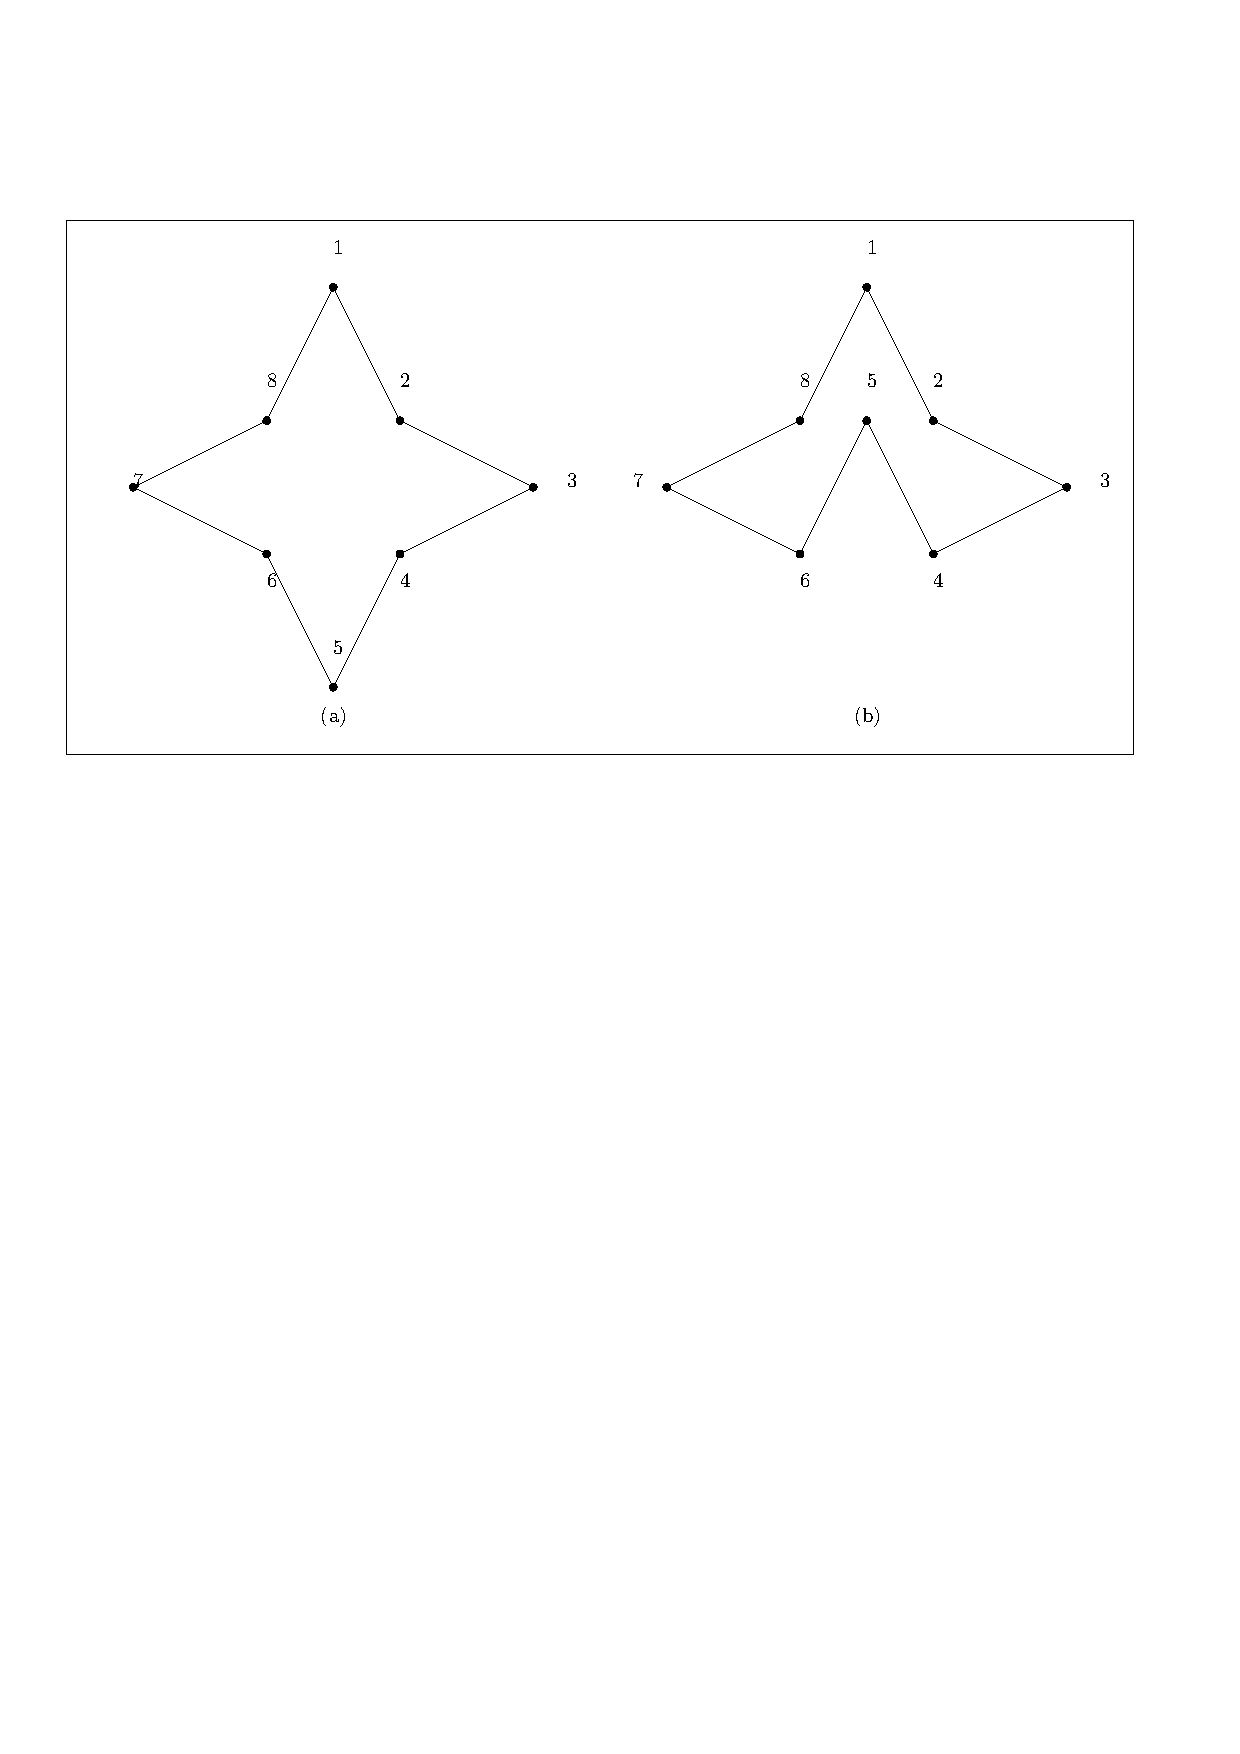
\includegraphics{graphics/twoEmbeddingsOfSameLinkage.pdf}
\end{center} 
\caption{(a) and (b) show a linkage in two embeddings.  Any realization of a path can be continuously moved without self-intersection to any other realizations.}
\label{fig:configuration-3}
\end{figure}

% \begin{figure}[!h]
% \begin{center}
% 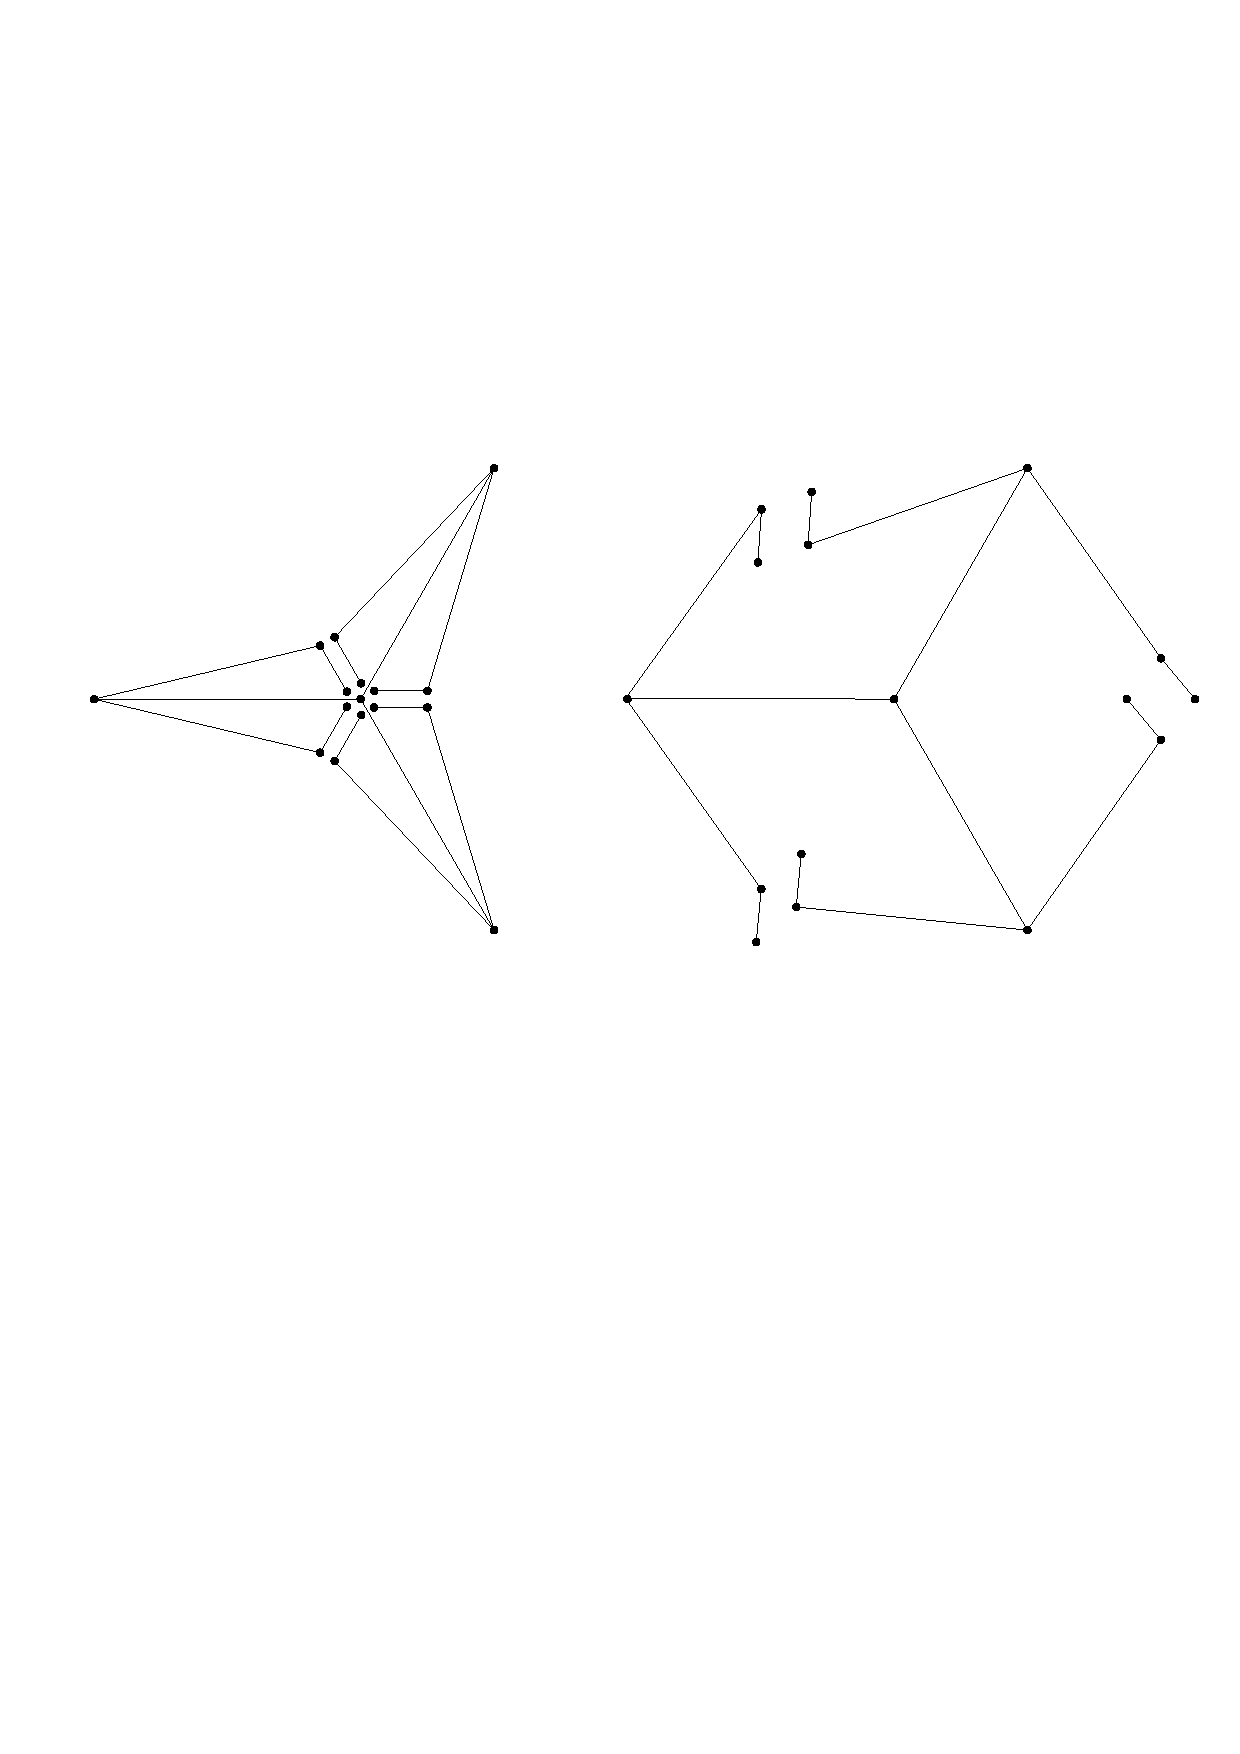
\includegraphics[scale=.75]{graphics/LockedConnellyLinkage.pdf}
% \end{center} 
% \caption{A linkage whose complete configuration space is discontinuous.  These two examples above 
% are two configurations of the same linkage that cannot continuously transform into the other 
% without edge crossing.}
% \label{fig:configuration-4}
% \end{figure}
% A \textit{reconfiguration} of a linkage whose graph is $G=(V,E)$ and length assignment is $\ell$ is 
% a continuous function $f: [0,1] \mapsto \bbr^{2 \cdot \vert V \vert}$ specifying a configuration of 
% the linkage for every $t \in [0,1]$ where length assignment $\ell$ is preserved, edges do not cross 
% and for every $\epsilon > 0$, there exists a $\delta > 0$ such that $\vert t_1 - t_2 \vert < 
% \delta$ implies 
% $$\left\vert f\left( t_1 \right) - f\left( t_2 \right) \right\vert < \epsilon$$

%(fig 1) insert a table of a graph and define a length assigment 
%(fig 2) insert a realization of (fig 1)
%(fig 3) insert a second realization of (fig 1)



%graph component of the linkage   the plane.  A linkage 
%\textit{embedding} is $L : V \mapsto 
%\bbR^{2}$.
% A \textit{linkage} is an ordered pair $G = (V,E)$ comprising of a set $V$ of vertices or nodes 
% together with a set $E$ of edges or lines. This definition is commonly used for graphs.  Mapping 
% the linkage $G$ into the plane is said to be the \textit{embedding}, i.e. $L : V \mapsto 
% \bbR^{2}$.  A length function correspond to a linkage, $l: E \mapsto \bbr^+$ gives a length to an 
% edge in the linkage.  If We consider a \textit{realization} of a linkage is range of $L$, i.e. 
% $L(V)$. If for every edge $(u,v) \in E$ such that $l\left( \left(u,v\right) \right) = \left\vert 
% L(u) - L(v) \right\vert$ is true, then $L$ is said to be a \textit{proper embedding} of $G$.
% \begin{figure}[h]
% \begin{center}
% 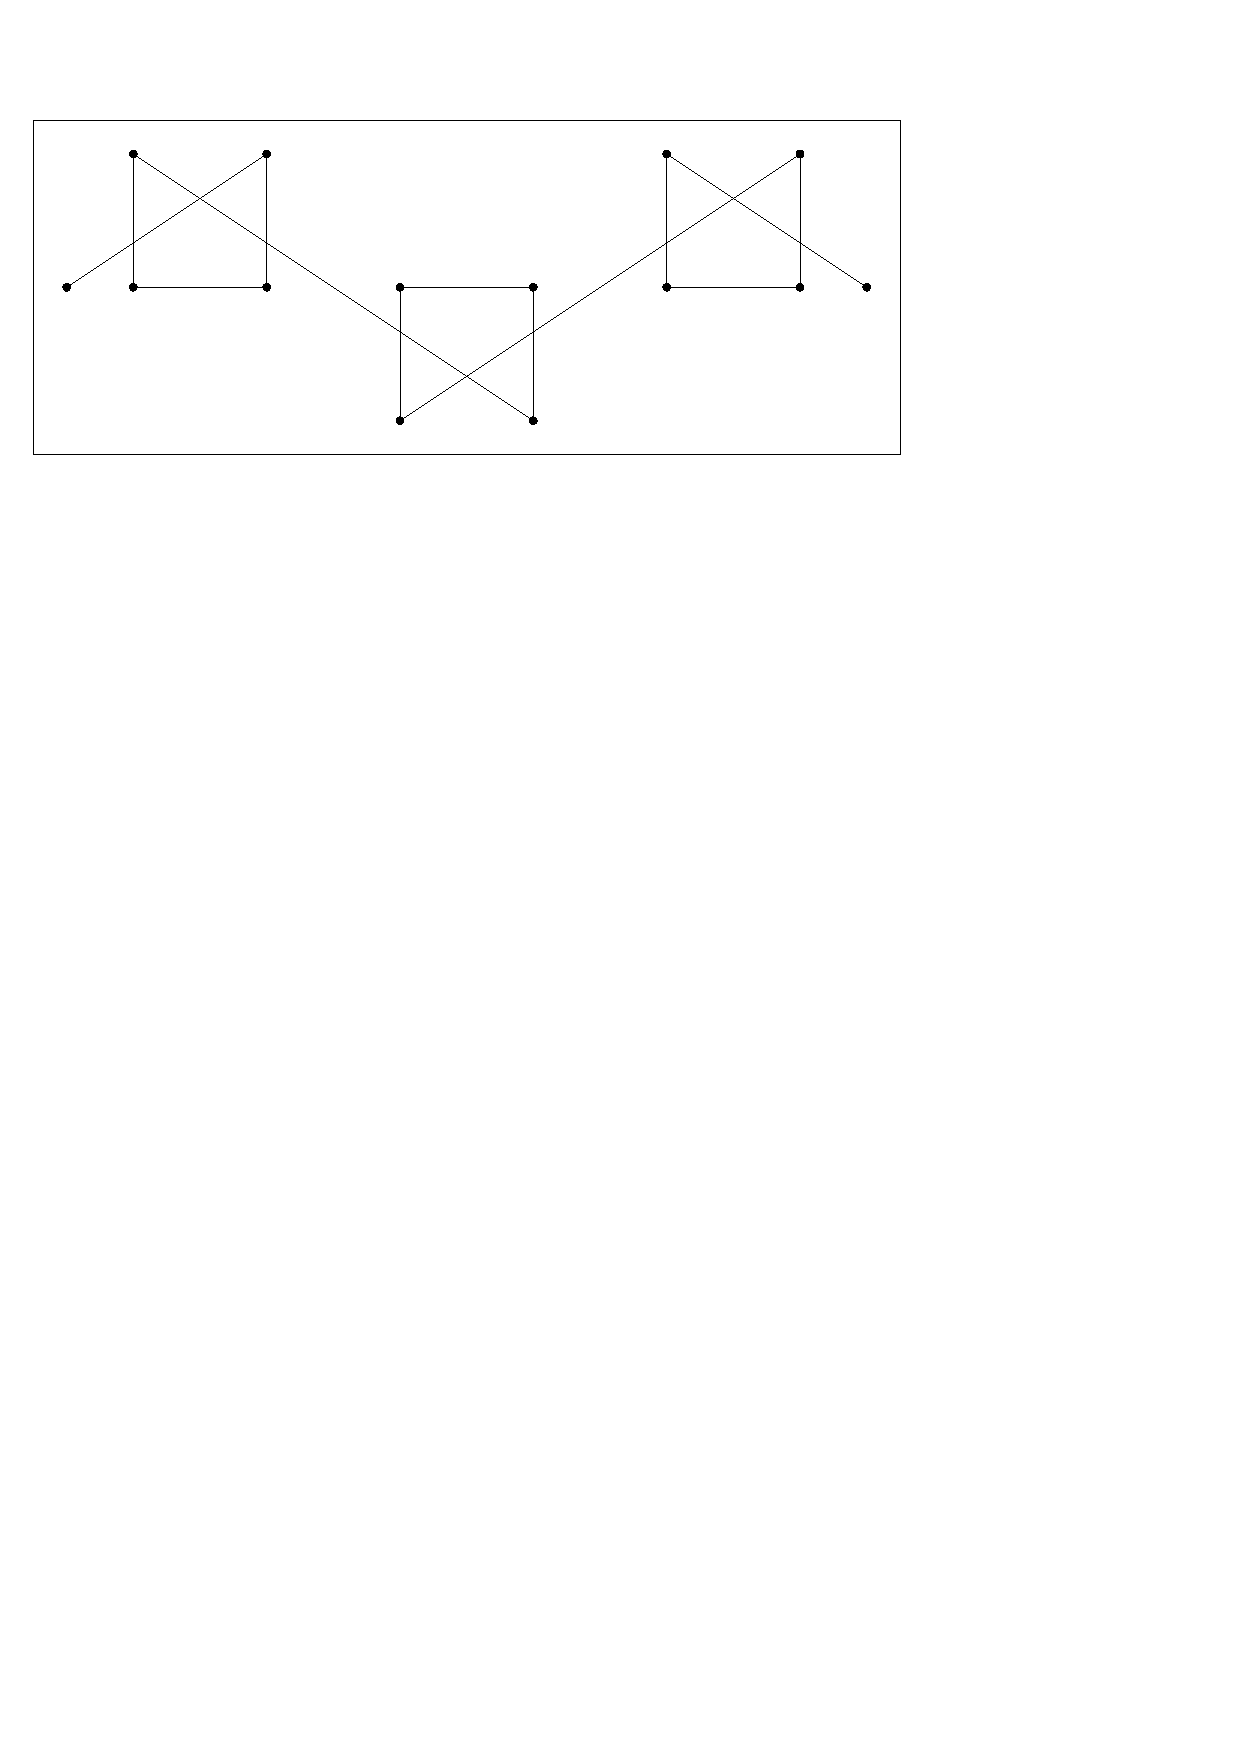
\includegraphics[scale=1]{graphics/crossingEdgeLinkage.pdf}
% \end{center} 
% \caption{A linkage where edges cross however it does not contain loops or multiple edges between 
% vertices.}
% \label{fig:linkage-3}
% \end{figure}
